\section{Ejercicio 2}

\subsection{Introducción}
\label{intro2}

\paragraph{}
El segundo problema que se propone en este trabajo práctico es el de, dado el trazado de calles de una ciudad compueto por esquinas y calles, decidir si es posible orientar las calles de forma tal que dadas dos esquinas cualesquiera resulte posible llegar de la primera a la segunda.\\
Se pide además que la complejidad temporal para este problema, medida con modelo uniforme, sea estrictamente menor a \Ode{n^4}.

\paragraph{}
Mediante un modelado con grafos, el problema puede ser representado de forma que los nodos de un grafo correspondan a las esquinas de la ciudad y las aristas a las calles que unen cada par de esquinas entre sí. \\
Entonces, para poder estudiar el problema con el modelo planteado es preciso primero establecer algunas definiciones:
\begin{itemize}
	\item \textbf{Def$_1$:} Un digrafo es ...
	\item \textbf{Def$_2$:} Un digrafo es \textit{fuertemente conexo} ...
	\item \textbf{Def$_3$:} Un grafo $G$ es \textit{fuertemente orientable} si existe una asignación de direcciones a los ejes del conjunto de ejes del grafo $G$ tal que el digrafo resultante es fuertemente conexo. 
	\item \textbf{Def$_4$:} \textit{un puente o arista de corte} es una arista que al eliminarse de un grafo incrementa el número de componentes conexos de éste. Equivalentemente, una arista es un puente si y sólo si no está contenido en ningún ciclo.
\end{itemize}

\paragraph{}
A partir de las definiciones anteriores, se desprende que la solución al problema en cuestión debe establecer si el grafo que modela el trazado de las calles es fuertemente orientable. Esto es, decidir si es posible para cada instancia del problema orientar el grafo que la modela, para obtener así un digrafo fuertemente conexo de modo que sea posible llegar desde cualquier nodo hasta cualquier otro.

\paragraph{}
El algoritmo desarrollado para dar solución al problema planteado recorre los ejes del grafo evaluando si es posible o no orientarlo para que cumpla lo requerido. Para ello, el mismo, se basa los algoritmos tradicionales de recorrido de grafos, como son BFS y DFS. En la sección contigua se expone de forma detallada las ideas que dieron lugar al algoritmo así como también el algoritmo en sí.

	
\subsection{Explicación}
\label{exp2}

\paragraph{}
Tal como se expuso en la introducción de este informe, el algoritmo a implementar debía ser capaz de decidir si el grafo que modela el trazado de la ciudad es orientable de modo que sea factible conectar cualquier nodo con cualquiera de los nodos restantes; es decir, que el grafo pueda orientarse para ser un digrafo fuertemente conexo.

\paragraph{}
Si se observa la definición de digrafo fuertemente conexo, ésta nos dice que para cualquier par de nodos \textit{a} y \textit{b}, existe al menos un camino orientado desde \textit{a} hasta \textit{b} y al menos otro desde \textit{b} hasta \textit{a}. Esto a su vez, asegura que el grafo es conexo, ya que para cada nodo del grafo existe un camino orientado hacia cada uno de los nodos restantes.

\paragraph{}
A partir del análisis anterior, es esperable que el algoritmo devuelva que no es posible orientar el trazado de calles de la ciudad según lo pedido cuando se da alguna de las siguientes situaciones: 
\begin{itemize}
	\item existe al menos un par de nodos que no están unidos por un camino de calles, con lo cual el grafo que modela el problema no es conexo;
	\item se puede llegar de una esquina \textit{a} a una esquina \textit{b}, pero no es posible realizar el camino inverso, con lo cual el grafo que modela el problema tiene un puente.
\end{itemize}

Buscando formalizar esta idea se recurrió a distintas fuentes bibliográficas hasta que finalmente se hayo el siguiente teorema:

\begin{quote}
\label{robbins}
\underline{Teorema: }\footnote{Demostrado por Robbins, 1939 - Gross \& Yellen "Graph Theory", Teorema 11.1.4}\\ \vspace{7pt}
Un grafo conexo G es fuertemente orientable si y solo si G no tiene puentes \footnote{Véase la demotración del teorema en la sección Anexos}.
\end{quote}

\paragraph{} 
Del teorema anterior, se confirma la idea expresada en el analisis previo según la cual, si se verifica que el grafo es inconexo o que el grafo es conexo pero tiene un puente, entonces no es posible darle una orientación para convertirlo en un digrafo fuertemente orientado.\\
En línea con está pensamiento, el algoritmo que resuelve el problema fue desarrollado con la idea la de verificar que el grafo sea conexo y no tenga puentes. Para ello, el algoritmo va recorriendo el grafo al igual que lo hace el algoritmo DFS\footnote{Para conocer el funcionamiento del algoritmo DFS véase \url{http://en.wikipedia.org/wiki/Depth-first_search}}, con la salvedad de que cuando llega a un nodo nuevo, además de marcarlo como visitado, guarda en él la lista de ejes que conforman el camino hasta ese punto. Seguidamente, elije de entre los vecinos del nodo actual (excluyendo al padre), el próximo nodo hacia el cual va a dirigirse. En este paso pueden darse dos situaciones: 
\begin{itemize}
	\item que el nodo elegido no esté marcado
	\item que el nodo ya esté marcado, y no sea el padre del nodo actual
\end{itemize}
En el primer caso, como el nodo no está marcado, el algoritmo lo toma y realiza un paso recursivo sobre el mismo nodo para de este modo seguir recorriendo el grafo en busca de puentes o de inconexiónes . Por el contrario, en el segundo caso, al encontrarse con un nodo marcado pero que no es el padre del nodo actual, el algoritmo se encuentra frente a la presencia de un ciclo, ya que acaba de encontrar un camino que le permite llegar nuevamente hacia un nodo ya visitado. De ser éste el caso, procede a guardar todos los ejes del ciclo en un conjunto en el cual se van registrando todos los ejes que formen parte de algún ciclo.
Así, el algoritmo procede hasta haber recorrido y marcado todos los nodos del grafo en cuyo caso finaliza devolviendo el número de nodos visitados y el conjunto con los ejes que pertenecen a algún ciclo. \\
Finalmente, si el numero de nodos recorridos es menor a la cantidad de nodos del grafo, eso significa que en algún punto el grafo no es conexo, y consecuentemente no es direccionable. De igual modo, si el conjunto de ejes que pertenecen a algún ciclo no es igual al conjunto de ejes del grafo, eso representa que existe al menos un eje que no forma parte de ningún ciclo, con lo cual es un puente y el grafo no puede ser dirigido según lo pedido.

A continuación se presenta el pseudocódigo del mismo, en el cuál usaremos a \textit{n} como la cantidad de esquinas (o nodos) y a \textit{m} como la cantidad de calles (o aristas): \\

\incmargin{1em}
\linesnumbered
\restylealgo{boxed}

void \textbf{dfs\_ciclos}(vertice: \nat, G: grafo\&, cuenta: \nat\&) \\
\begin{algorithm}[H]
	\SetKw{Orden}{Complejidad:}
	\Orden{\Ode{m*n*log(n)}}
	\BlankLine
	G.info[vertice].ejesHasta $=$ G.info[G.info[vertice].padre].ejesHasta \tcp*{\Ode{tam(ejesHasta)} $\subseteq$ \Ode{n}}
	G.info[vertice].ejesHasta.insert(eje(G,vertice,G.info[vertice].padre)) \tcp*{\Ode{1}}
	cuenta $\leftarrow$ cuenta + 1 \tcp*{\Ode{1}}
	G.info[vertice].ejesHasta $\leftarrow$ G.info[G.info[vertice].padre].ejesHasta \tcp*{\Ode{n}}
	G.info[vertice].visitado $\leftarrow$ true \tcp*{\Ode{1}}
	\BlankLine
	\textbf{var} it*: it\_secu \textless \nat \textgreater \ $\leftarrow $ G.info[vertice].vecinos.begin() \tcp*{\Ode{1}}
	\BlankLine
	\For{(it; it $\neq$ G.info[vertice].vecinos.end(); it++)}{ 
		%if
		\eIf{(G.info[*it].visitado $==$ false)\tcp*{\Ode{1}}}
			{G.info[*it].padre $\leftarrow$ vertice \tcp*{\Ode{1}}
			dfs\_ciclos(*it,G,cuenta)}
		%else	
			%if
			{\lIf{(G.info[vertice].padre $\neq$ (*it))\tcp*{\Ode{1}}}
				{\BlankLine
insertarResta(G.ejesUsados,G.info[vertice].ejesHasta\\
,G.info[*it].ejesHasta)\tcp*{\Ode{n*log(n)}}
	G.ejesUsados.insert(eje(G,*it,vertice))\tcp*{\Ode{log(tam(ejesUsados))} $\subseteq$ \Ode{log(m)} $\subseteq$ \Ode{log(n^2)} $\subseteq$ \Ode{log(n)}}}}}

	\caption{Pseudocódigo de la función \textit{dfs\_ciclos} con el costo de cada instrucción en el modelo uniforme}
\end{algorithm}

\vspace{11pt}

\incmargin{1em}
\linesnumbered
\restylealgo{boxed}

void \textbf{insertarResta}(ejesEnCilos: set$<$int$>$, vEjesHasta: set$<$int$>$, wEjesHasta: set$<$int$>$) \\
\begin{algorithm}[H]
	\SetKw{Orden}{Complejidad:}
	\Orden{\Ode{n.log(n)}}
	\BlankLine
	\For{(it = vEjesHasta.begin(), it $\neq$ vEjesHasta.end(), it++)\tcp*{\Ode{tam(vEjesHasta)} $\subseteq$  \Ode{n} }} {
		\lIf{ (wEjesHasta.count(*it) == 0)} {ejesEnCiclos.insert(*it)\tcp*{\Ode{log(tam(wEjesHasta))} $\subseteq$ \Ode{log(n)}}}
	}
	
	\caption{Pseudocódigo de la función \textit{insertarResta}}
\end{algorithm}


\subsection{Análisis de la complejidad del algoritmo}
\label{complejidad2}

\paragraph{}
Para el análisis de la complejidad de este algoritmo, vamos a remitirnos a los pseudocódigos de las funciones \textit{dfs\_ciclos} y \textit{insertarResta} adjuntos en las secciones [\ref{exp2}] y [\ref{PseudoInsResta}] respectivamente. En este caso se utilizará la misma notación para la cantidad de nodos y aristas que se utilizó en los pseudocódigos de la sección [\ref{exp2}].

\paragraph{}
Si se observan las distintas complejidades que se dan dentro del algoritmo, se puede ver algunas que sobresalen sobre el resto. Es en estas en las que recae la complejidad total del algoritmo, por lo cuál el análisis se realizará sobre estas instrucciones.\\
Como primer caso de análisis, se puede observar en la tercer línea que la complejidad de la instrucción es \Ode{n}. Esto se debe a que la asignación de conjuntos implementada en la \textit{STL} tiene esta complejidad (destrucción y copia de un conjunto).

\paragraph{}
La siguiente complejidad a analizar es la referente al ciclo \textit{for}. Como hay una llamada recursiva dentro, vamos a hacer un análisis más arraigado a la idea en sí de DFS que al pseudocódigo tal como está. Si pensamos en cómo funciona DFS, sabemos que este visitará a cada nodo a lo sumo una vez (estrictamente una única vez en caso que el grafo sea conexo). Por lo que si se observa detalladamente dentro del \textit{for}, la sentencia \textit{if} sólo se ejecutará\footnote{Se entiende por ``ejecutará'' a que la condición de \true.} n veces. Dentro de esa sentencia, sólo se hacen operaciones de complejidad \Ode{1} y una llamada recursiva. Dicha llamada recursiva en realidad puede pensarse como \Ode{1} ya que si la función fuese iterativa, la recursión equivale a hacer un ``apilar'' de un nodo, y esto cuesta efectivamente \Ode{1}.

\paragraph{}
Ahora falta ver cuántas veces se ejecutará la otra parte de la sentencia condicional, es decir, el  \textit{else}. La complejidad de ejecutar una vez esta parte de la sentencia está dada por el llamado a la función \textit{insertarResta}, la cuál es \Ode{n*log(n)}. Si se analiza profundamente, se va a entrar a este lado de la sentencia siempre que se intente visitar a un nodo que ya fue visitado. En otras palabras y siendo un poco más formal, a cada nodo a lo sumo se va a intentar entrar tantas veces como ejes incidan en él, es decir, d(v) veces (donde v es algún nodo perteneciente al grafo). La primer vez que se lo visite entrará en el \textit{if} y el resto de las d(v)-1 veces entrará en el \textit{else}.\\
Sabemos que $\sum_{i=1}^{n} d(v_i) = 2*m$. Como el grado de un nodo puede ser a lo sumo n-1, entonces para cada nodo voy a estar ejecutando una vez el \textit{if} y n-2 veces el \textit{else}. Si contamos con que la complejidad de ejecutar el \textit{if} es \Ode{1} y la del \textit{else} es \Ode{n*log(n)} y que por cada nodo se van a ejecutar una vez y n-2 veces cada una respectivamente (sin olvidarnos de la sumatoria antes mencionada), entonces se puede decir que en total, la complejidad de ejecutar el \textit{if} es \Ode{n} y la del \textit{else} es \Ode{2*m*n*log(n)} $==$ \Ode{m*n*log(n)}.

\paragraph{}
Finalmente entonces, la complejidad total del algoritmo es \Ode{n + m*n*log(n)} $\subseteq$ \Ode{m*n*log(n)}.

\paragraph{}
Hasta aquí hicimos el análisis suponiendo que la complejidad de \textit{insertarResta} era \Ode{n*log(n)}. Pero para que la complejidad quede bien justificada, queda analizar que dicho algoritmo cumpla esta complejidad.\\
La función consta de tres operaciones costosas. En primer instancia está el ciclo \textit{for}, el cuál se va a ejecutar a lo sumo n-1 veces. Esto se debe a que dicho conjunto hace referencia a los ejes que pertenecen al camino simple raiz$\rightarrow$ $v_i$ (con $v_i$ cualquiera de los vértices pertenecientes al grafo original), por lo que la cantidad de ejes es a lo sumo n-1, es decir, \Ode{n}. Luego, hay una sentencia condicional, para la cuál se hace una búsqueda sobre un conjunto, el cuál, al igual que el conjunto perteneciente al ciclo, tiene a lo sumo n-1 ejes por lo que dicha complejidad es \Ode{log(n)}. Finalmente, se realiza una inserción en otro conjunto. Este conjunto es el que va acumulando todos los ejes del grafo original que pertenecen a algún ciclo, por lo que a lo sumo puede contener todos los ejes del grafo, es decir m, por lo que la inserción cuesta \Ode{log(m)}. Pero m es a lo sumo $n^2$, es decir que: \Ode{log(m)} $\subseteq$ \Ode{log(n^2)} $==$ \Ode{log(n^2)} (por propiedades del logaritmo y de $O$). Es decir que por cada eje del primer conjunto, se ejecutan dos instrucciones de complejidad \Ode{log(n)}, por lo que la complejidad final de la función \textit{insertarResta} sería \Ode{n*log(n)}.


\subsection{Detalles de implementación}
\label{imp2}

\paragraph{}
Dentro de la carpeta \textit{./ej2/}, se puede encontrar el archivo ejecutable \textit{ejercicio\_2} compilado para GNU-Linux, el cual resuelve el problema anteriormente descripto. Este programa se ejecuta por consola mediante el comando \texttt{./ejercicio\_2}, y recibe como parámetro los archivos de entrada \textit{".in"} a procesar. Puede recibir tantos nombres de archivo como se desee, pero en caso de no recibir ninguno, el programa procesará el archivo \textit{Tp2Ej2.in} que se encuentra incluído dentro de la misma carpeta. \\
Una vez ejecutado, el algoritmo procesa la cola de archivos que recibió como parámertos de a uno por vez generando para cada uno de ellos dos archivos:
	\begin{itemize}
		\item{Un archivo \textit{".out"} omónimo con la solucion a cada instancia del problema contenidos en el archivo de entrada.}
		\item{Un archivo omónimo con el sufijo \textit{"\_grafico.out"}, en el cual registra para cada instancia la cantidad de ejes del grafo que modela el problema y el tiempo promedio que tardó el algoritmo en resolverlo. Este archivo tiene objetivo facilitar la tarea de cargar los datos en el programa de análisis gráfico \textit{QtiPlot}}.
	\end{itemize}

Ambos archivos son guardados en la misma carpeta de origen que la del archivo \textit{'.in'}.

\paragraph{}		
Por otra parte, en la misma carpeta, hay un Makefile el cual permite recompilar los archivos ejecutables con tan solo ejecutar el comando \texttt{make} en la consola. Además, ejecutando el comando \texttt{make clean} se pueden eliminar los archivos ejecutables y todos los archivos contenidos en la caperta \textit{'test/'}. 

\paragraph{}
Luego, en la carpeta \textit{./ej2/sources} se encuentran el codigo fuente dell ejecutable antes descripto escrito en lenguaje C++ y cometando para simplificar la comprensión. Asímismo, en esta carpeta se puede hallar el script \textit{input\_gen2.py} para ser ejecutado desde la consola con el intérprete de Python mediante el comando \texttt{python input\_gen2.py} . Al correr este programa se despliega un menú de opciones para generar distintos tipos de archivos \textit{".in"} para ser resueltos por el ejecutable \textit{ejercicio\_2}. Una vez elegido el tipo de entrada a crear, el programa solicita que se ingrese la cantidad de casos a generar. Acto seguido guarda el archivo generado en la carpeta \textit{./ej2/tests}. Se recomienda, una vez generados varios archivos de prueba, ejecutar el comando \texttt{./ejercicio\_2 tests/} para que el programa \textit{ejercicio\_2} resuelva todos los archivos de ese directorio con una única ejecución.

\paragraph{}
Finalmente, en \textit{./ej2/} se hayan los archivos \textit{.Tp2Ej2.in} y \textit{Tp2Ej2.out} que vienen junto con en el enunciado de este Trabajo Práctico, y se haya también la carpeta \textit{./ej2/pruebas\_graficos} la cual contiene los archivos \textit{".in"} generados para la exprimentacion que se presenta en este informe, junto con sus correspondientes archivos \textit{".out"} y sus gráficos de \textit{m} vs. \textit{Tiempo}.


\subsection{Resultados}
\label{res2}

\paragraph{}
El programa \textit{input\_gen2.py} fue desarrollado para poder crear cinco casos posibles de archivos input de distintas características, cada uno con un número de instancias dado por el usuario. Allí, cada instancia corresponde a un posible trazado de la ciudad caracterizado por la cantidad de esquinas y la cantidad de calles adyacentes a cada una de ellas. \\
A continuación se describen cuáles son esos casos y se explica brevemente que se esperaba observar en cada uno de ellos\footnote{Cabe aclarar que en todos los casos, tanto el número de nodos, como el grado de los mismos se generan de forma aleatoria, pero siempre dentro de los rangos establecidos por cada uno de los casos.}:
	\begin{itemize}
		\item[\texttt{a.-}]{\texttt{Casos con $0 \leq n \leq 100$ y $d(v_i) \geq\ \frac{n-1}{2},\ \forall\ 0 \leq i \leq n$:} \\
		Se pensó en este tipo de casos para poder evaluar el comportamiento del algoritmo frente al que se presupone el peor caso posible (ya que en este caso están incluídos los grafos completos). Este es, el de instancias donde los grafos que las modelen tengan un gran número de nodos y sea sumamente densos (ya que cada nodo tiene al menos $\frac{n-1}{2}$ nodos incidentes).} 
		\item[\texttt{b.-}]{\texttt{Casos con $0 \leq n \leq 100$ y $d(v_i) \leq\ \frac{n-1}{2},\ \forall\ 0 \leq i \leq n$:} \\
		Se pensó en este tipo de casos para poder evaluar el comportamiento del algoritmo frente grafos con un gran número de nodos, pero no tan densos como el del caso previo (ya que cada nodo tiene a lo sumo $\frac{n-1}{2}$ nodos incidentes).} 
		\item[\texttt{c.-}]{\texttt{Casos con $0 \leq n \leq 10$ y $d(v_i) \geq\ \frac{n-1}{2},\ \forall\ 0 \leq i \leq n$:} \\
		Se pensó en este tipo de casos para poder evaluar el comportamiento del algoritmo frente a grafos con un reducido número de nodos, pero con muchas conexiones entre sí.}
		\item[\texttt{d.-}]{\texttt{Casos con $0 \leq n \leq 10$ y $d(v_i) \leq\ \frac{n-1}{2},\ \forall\ 0 \leq i \leq n$:} \\
		Se pensó en este tipo de casos para poder evaluar el comportamiento del algoritmo frente al que se presupone el mejor caso posible. Este es el de grafos con un pequeño número de nodos y escazamente densos.} 
		\item[\texttt{e.-}]{\texttt{Casos con $0 \leq n \leq 50$ y $d(v_i) \leq\ \frac{n-1}{2},$ ó $d(v_i) \geq\ \frac{n-1}{2},\ \forall\ 0 \leq i \leq n$:} \\ 
		Finalmente, se pensó en este caso, para ver el comportamiento del algoritmo frente al caso de grafos con un número de nodos medio y con una densidad alta o baja establecida de manera aleatoria.}
	\end{itemize}  

\paragraph{}
Mediante cada uno de estos casos se buscó estudiar el comportamiento del algoritmo para luego establecer su complejidad real, valiéndose para ello de la medición del tiempo (en microsegundos) que demora el algoritmo en resolver el cada instancia del problema. 
No obstante, puesto que este tipo de medición sufre de varias impresiciones propias del instrumento usado para medir se debió buscar una manera de acotar ese error\footnote{Esto se debe a que mientras el ordenador está contando el tiempo de ejecución pueden tener lugar varios eventos como pueden ser las interrupciones al sistema operativo, llamados a memoria, etc., que detengan la ejecución del algoritmo en cuestión, pero no así la del contador de tiempo.}. \\
Para subsanar este inconveniente, en cada uno de los archivos de pruebas utilizados durante la experimentación, se ejecutaron cien veces cada una de sus instancias, acumulando los tiempos de cada ejecución y calculando luego el tiempo promedio. De esta forma, se logró obtener un valor de estable y representativo del tiempo requerido por el algoritmo para resolver cada una de las intancias propuestas.

\paragraph{}
Seguidamente, y previo al momento de la experimentación, se formularon varias hipótesis en cuanto a cuál era el comportamiento esperable del algoritmo frente a cada uno de los tipos de inputs elegidos para su estudio. Las mismas son presentadas a continuación:
	\begin{itemize}
		\item[1)]{Tal como se explicó en la sección [\ref{complejidad2}], la parte mas costosa del algoritmo está dada por la rama \textit{else} del ciclo \textit{for} del algoritmo \textit{dfs\_ciclos}. Esta rama es accedida cuando alguna arista del nodo sobre el que se está iterando incide sobre un nodo ya recorrido distinto del padre; es decir, cuando se encuentra una arista que es parte de algún ciclo. Luego si se desea estudiar el caso en que el algoritmo tiene la peor complejidad posible, es deseable que para el grafo a procesar cuente con muchos ciclos; más aún que el grafo sea completo. Por estos motivos, es de esperase que los archivos del caso \texttt{a} sean los que tarden más tiempo en resolverse, ya que son los de instancias con un gran número de nodos y una alta densidad.}
		\item[2)]{Del mismo modo, y debido a su gran cantidad de nodos, resulta esperable que las instancias de los archivos del caso \texttt{b} tarde un tiempo considerable en resolverse, aunque menor que los del caso anterior.} 
		\item[3)]{Finalmente, se podría presuponer que debido a que tienen un n pequeño, en los grafos de las instancias de los archivos del caso \texttt{c} y \texttt{d} el grado de cada nodo también será un valor chico, disminuyendo así la posibilidad de formar ciclos y consecuentemente disminuyendo la posibilidad de entrar en la rama costosa del algoritmo. En conclusión, se puede pensar a priori que el algoritmo para estos casos resolverá las instancias a una velocidad aceptable/acelerada.}
	\end{itemize}

\paragraph{}
En lo que respecta a la experimentación propiamente dicha, se generaron cinco archivos correspondientes a cada uno de los tipos descriptos, cada uno con cien instancias (posibles trazados de la ciudad) del problema. Seguidamente, se procedió a correrlos con el programa \textit{ejercicio\_2},  obteniéndose para cada uno de ellos un archivo \textit{"NombreDeArchivo.out"} y un archivo \textit{"NombreDeArchivo\_grafico.out"}; siendo este último el archivo en el cual se registraron de cada instancia del archivo original, la cantidad de aristas (\textit{m}) y el tiempo promedio necesario para ser resuelta por el algoritmo. \\
Finalmente, haciendo uso de esos archivos se generaron, usando el programa de análisis gráfico \textit{QtiPlot}, diversos gráficos de \textit{m} vs. \textit{Tiempo} en los cuales se contrasta la curva de resultados con una función 
	$$f: \nat_0 \rightarrow \real / f(n)\ =\ c * m * \sqrt{m} * log(m),\ c \in \real^+$$
para poder estudiar si la complejidad real se ajusta a la complejidad teórica.

\paragraph{}
A continuación se presentan los gráficos realizados para cada caso:

\begin{center}
\vspace*{1.5cm}
\label{graficoA}
\hspace*{-2.1cm}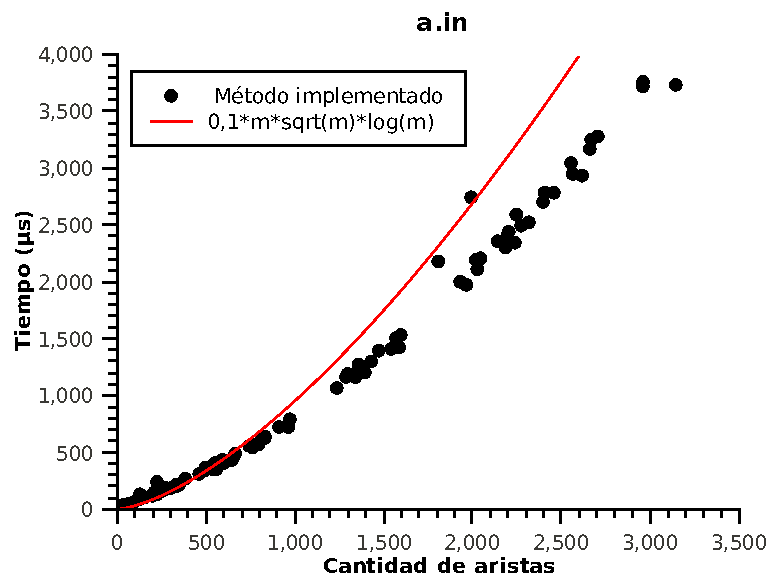
\includegraphics[scale = 0.9]{../ej2/pruebas_graficos/GraphA.pdf} \\
\underline{Gráfico A} Gráfico de \textit{Cantidad de ejes vs. Tiempo} del caso A

\vspace*{1.5cm}
\label{graficoB}
\hspace*{-2.1cm}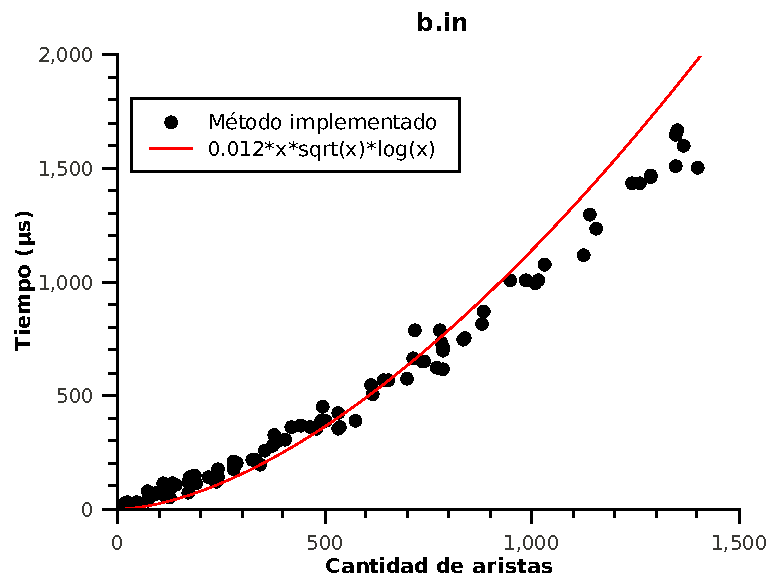
\includegraphics[scale = 0.9]{../ej2/pruebas_graficos/GraphB.pdf} \\
\underline{Gráfico B} Gráfico de \textit{Cantidad de ejes vs. Tiempo} del caso B

\vspace*{1.5cm}
\label{graficoC}
\hspace*{-2.1cm}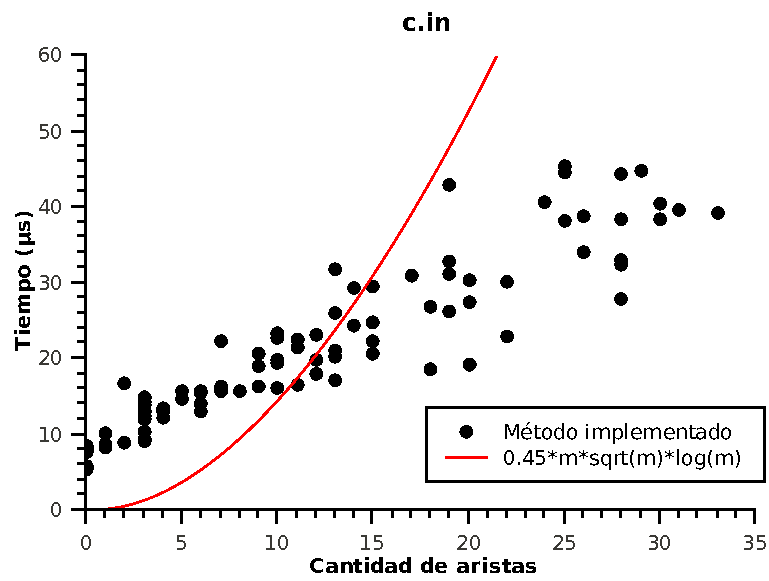
\includegraphics[scale = 0.9]{../ej2/pruebas_graficos/GraphC.pdf} \\
\underline{Gráfico C} Gráfico de \textit{Cantidad de ejes vs. Tiempo} del caso C

\vspace*{1.5cm}
\label{graficoD}
\hspace*{-2.1cm}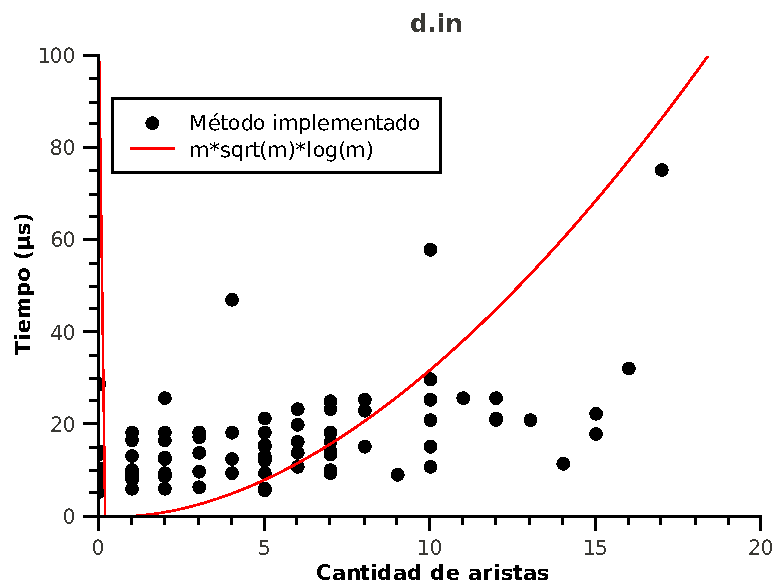
\includegraphics[scale = 0.9]{../ej2/pruebas_graficos/GraphD.pdf} \\
\underline{Gráfico D} Gráfico de \textit{Cantidad de ejes vs. Tiempo} del caso D

\vspace*{1.5cm}
\label{graficoE}
\hspace*{-2.1cm}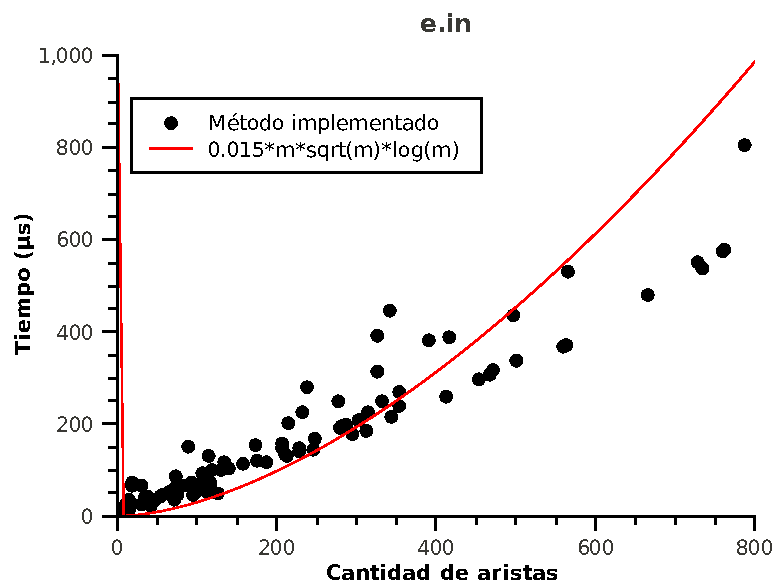
\includegraphics[scale = 0.9]{../ej2/pruebas_graficos/GraphE.pdf} \\
\underline{Gráfico E} Gráfico de \textit{Cantidad de ejes vs. Tiempo} del caso E
\end{center}

\clearpage 


\subsection{Debate}
\label{deb2}

\paragraph{}
Como primera observación de los gráficos expuestos en la sección anterior, cabe decir que la complejidad real se ajustó a la complejidad teórica, ya que en todos los casos se pudo hallar una constante $c \in\ \real$ tal que a partir de algún $n_0$ el gráfico de $c*m*\sqrt{m}*log(m)$ pasa a acotar superiormente a la cantidad de operaciones realizadas por el algoritmo.

\paragraph{}
En lo que respecta a la las hipótesis postuladas en la sección [\ref{res2}], analicemos una a una su veracidad en función de los gráficos obtenidos.\\
Cotejando el gráfico \ref{graficoA} con los gráficos restantes se corrobora la hipótesis 1 ya que para las instancias del caso \texttt{a} los microsegundos consumidos por el algoritmo son del orden de los 3700$\mu$ s aproximadamente, mientras que el del caso más próximo en tiempo insumido (el caso \texttt{b}) no traspasa la barrera de los 1700$\mu$s.\\
De esta última observación, también se puede inferir que la hipótesis 2 se ve corroborada de manera empírica.

\paragraph{}
En cuanto a la hipótesis 3, la comparación de los gráficos \ref{graficoC} y \ref{graficoD} contra los de los gráficos \ref{graficoA} y \ref{graficoB} evidencia que los tiempos necesarios para resolver los archivos de los primeros son significativamente menor a los tiempos necesarios para resolver los archivos de los segundos. Esto en principio, parecería corroborar la hipótesis 3.\\
No obstante, se puede apreciar también que, si bien se puede encontrar una curva que acote estos gráficos a partir de un cierto punto, esta curva no se ajusta tan bien como las curvas que acotan los gráficos \ref{graficoA} y \ref{graficoB}. Asímismo, se puede ver que la curva de \textit{m vs. Tiempo} de los gráficos \ref{graficoC} y \ref{graficoD} es mucho más irregular y oscilante que la de los gráficos \ref{graficoA} y \ref{graficoB}. Una comparación de los primeros con el gráfico \ref{graficoE}, arroja resultados similares, ya que si bien tiene valores de tiempo menor, este último gráfico se asemeja más a los gráficos de \ref{graficoA} y \ref{graficoB}.\\
En síntesis, si bien el resultado de la hipótesis 3 se cumple, las causas por las que esto ocurre no resultan del todo claras, y en principio no resulta correcto afirmar la hipótesis de que un número pequeño de nodos disminuye la posibilidad de formar ciclos y consecuentemente la posibilidad de entrar en la rama costosa del algoritmo.


\subsection{Conclusiones}
\label{conc2}
En base analizado en la sección [\ref{deb2}], cabe remarcar como conclusión el hecho de que la complejidad medida en la realidad se asemeje bastante a las complejidades teóricas estimadas. Asímismo, el hecho de que las hipótesis 1 y 2 fueran corroboradas en base a los resultados arrojados por la experimentación. \\ 
Por último, se puede concluir que el hecho de que si bien se cumple el resultado de la hipótesis 3, las causas por lo que esto ocurre no se evidencian a partir de la experimentación. En consecuencia, no se puede afirmar la hipóteisis 3, pero tampoco se la puede descartar llanamente. Como hipótesis alternativa se puede plantear que la oscilación en las curvas de los gráficos  \ref{graficoC} y \ref{graficoD}, o bien se debe al pequeño número de nodos del grafo (tal como se postuló en la hipótesis 3), o bien puede deberse al error producido al medir el tiempo aún pese haber tomado como medición representativa el tiempo promedio.


